\bgroup{}

\chapter{Evaluation}\label{cha:evaluation}
This chapter explains the evaluation process of the developed application described in \cref{cha:implementation}. Predefined examples measure the performance of the program using sets of data with a determined solution and analyze the steps needed to achieve said result. The examples simulate different types of use cases, which, in effect, exposes the strengths and weaknesses of the implementation.

\section{Subjectivity}
As the application should be flexible enough to deal with varying levels of sound perception, the evaluation process needs multiple examples to test how the program performs in different situations. All of these test cases need a common established standard of subjectivity to evaluate the application objectively.

The approach chosen in this project to form this specification of subjectivity is to construct sets of data consisting of timbrally differentiating groups of sound. Although distinction by timbre might be subjective in itself, user-derived groups of sound from Freesound, together with the author choosing the groups, will act as the judge in this case. Freesound supports sound pack configurations defined by their users~\cite{freesound:packs}, which the test cases, in turn, take advantage of as building blocks. The examples utilize various packs to either model a more closely resembled sound landscape, with say similar-sounding synthesizer sounds, or a more contrasting one, e.g., with drums and piano sounds. Most of the packs have descriptive tags, meaning the labels of the annotated sounds are what the sound represents: `gunshot', `guitar sound', or similar. Even though the application's primary goal is to deal with subjective tags, the descriptive tags are applicable for test data, as they are, in a sense, generally agreed upon subjective tags. Some sound waves classify as piano sounds to humans while others do not, but the infinite amount of interlying sounds keeps the separating border open to debate.

\section{Measurement}\label{sec:measurement}
The unit used for grading in the evaluation will be the number of user interactions needed to reconstruct the test data interpretation until each sample resides in its appointed group. Such rearrangements occur every time the user chooses to retag a sound, thus creating more groups and changing the structure of existing ones (see \cref{sub:modifying_groups} for more details). This strategy implies that the best-case scenario will be with zero corrections made by the user, which occurs when the starting \emph{Mean Shift} algorithm (\cref{sub:mean_shift}) finds the right number of groups immediately. The more modifications needed from the user, the worse the performance rating becomes, signifying that the clustering logic only discovering a single group when the user wants each sound to be in its group is the worst-case scenario.

When correcting sounds with erroneous tags, the order of which this is performed matters. Similar to how a chess opening alters the course of the game, the sound initially revised affects the rest of the modification process, which may conclude in a path with fewer or more total adjustments needed. Choosing to verify sounds as they become tagged or leaving them be also plays a vital role in how the application functions further on. This variation makes it difficult to measure all potential outcomes in complex use cases and settle on a final score.

\newpage\section{Case 1 – Rudimentary}
In this introductory example, sounds from two unconnected packs will make up the test data. The first pack of sound, \emph{Box Drum}~\cite{pack:1904}, consists of 15 samples produced by hitting a large metallic box under a bridge. \emph{Metal Guitar loops Un trimmed 150BPM}~\cite{pack:19793} is the second pack used and contains ten, as hinted by the name, distorted guitar sounds all played at the same speed.

The goal in this example will be to have the sounds separated into two groups, having the box drum sounds tagged as \textbf{Box}, and the metal guitar sounds labeled with \textbf{Guitar}. Loading the test data into the application, one can see that opening groupings done by the program coheres with the wanted result; all the box sounds are in one group, and the guitar sounds in another.
\begin{figure}[ht]
    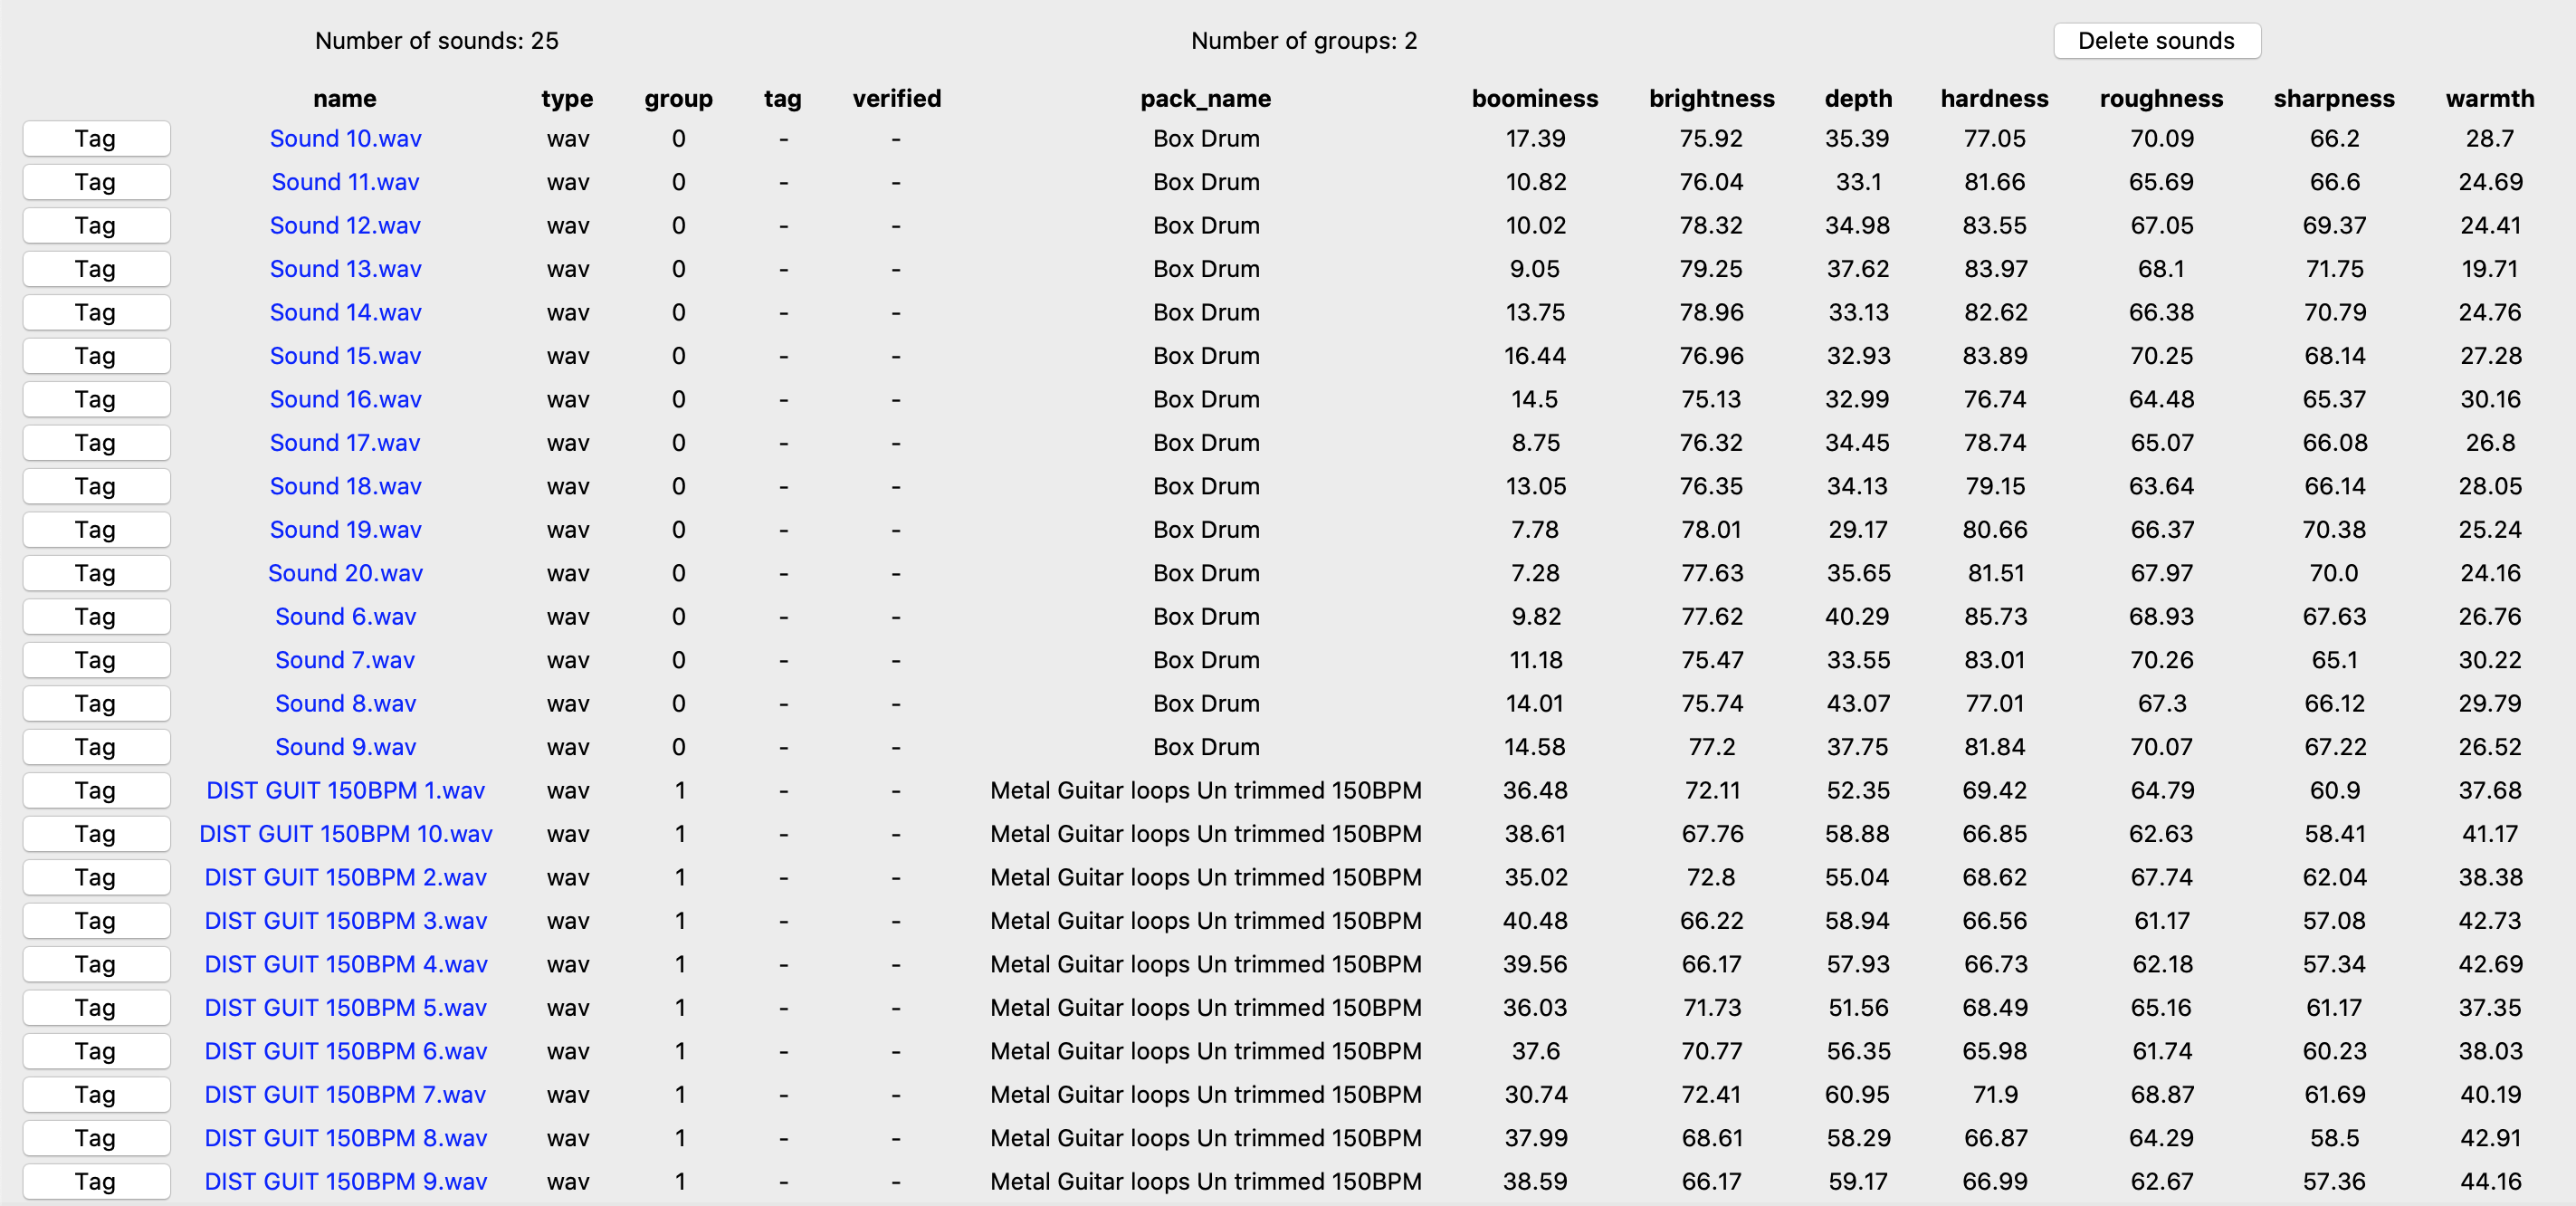
\includegraphics[width=\textwidth]{figures/case_1/initial}
    \caption{Case 1 test data initially loaded into the application.}\label{fig:case_1/initial}
\end{figure}

Worth noting for both packs is that the sound source remains constant throughout all samples, hence the sounds being comparatively similar sounding in themselves, mostly varying in rhythm, intensity, and placement. The calculated timbral characteristics reflect this auditory closeness, with the average range between the maximum and minimum values shown in \cref{tab:case_1} being a relatively small value.
\begin{table}[ht]
    \caption[Case 1 timbral characteristics max and min ranges]{Case 1 timbral characteristics maximum and minimum value ranges}\label{tab:case_1}
    \begin{tabular*}{\textwidth}{@{\extracolsep{\fill}}lrr}
        \toprule
        & \emph{Box Drum} & \emph{Metal Guitar loops Un trimmed 150BPM} \\
        \midrule
        \textbf{boominess} & 10.11 & 9.74 \\
        \textbf{brightness} & 4.12 & 6.63 \\
        \textbf{depth} & 13.89 & 9.39 \\
        \textbf{hardness} & 8.98 & 5.92 \\
        \textbf{roughness} & 6.63 & 7.70 \\
        \textbf{sharpness} & 6.66 & 4.96 \\
        \textbf{warmth} & 10.51 & 6.81 \\
        \midrule
        Average & 8.70 & 7.31 \\
        \bottomrule
    \end{tabular*}
\end{table}

This example falls under the best-case scenario, as the user needs to make \textbf{no group modifications} to give each sound its proper tag. Labeling one sound from each pack with the corresponding tag correctly tags the remaining sounds as well, via the program's automatic tagging procedure.
\begin{figure}[ht]
    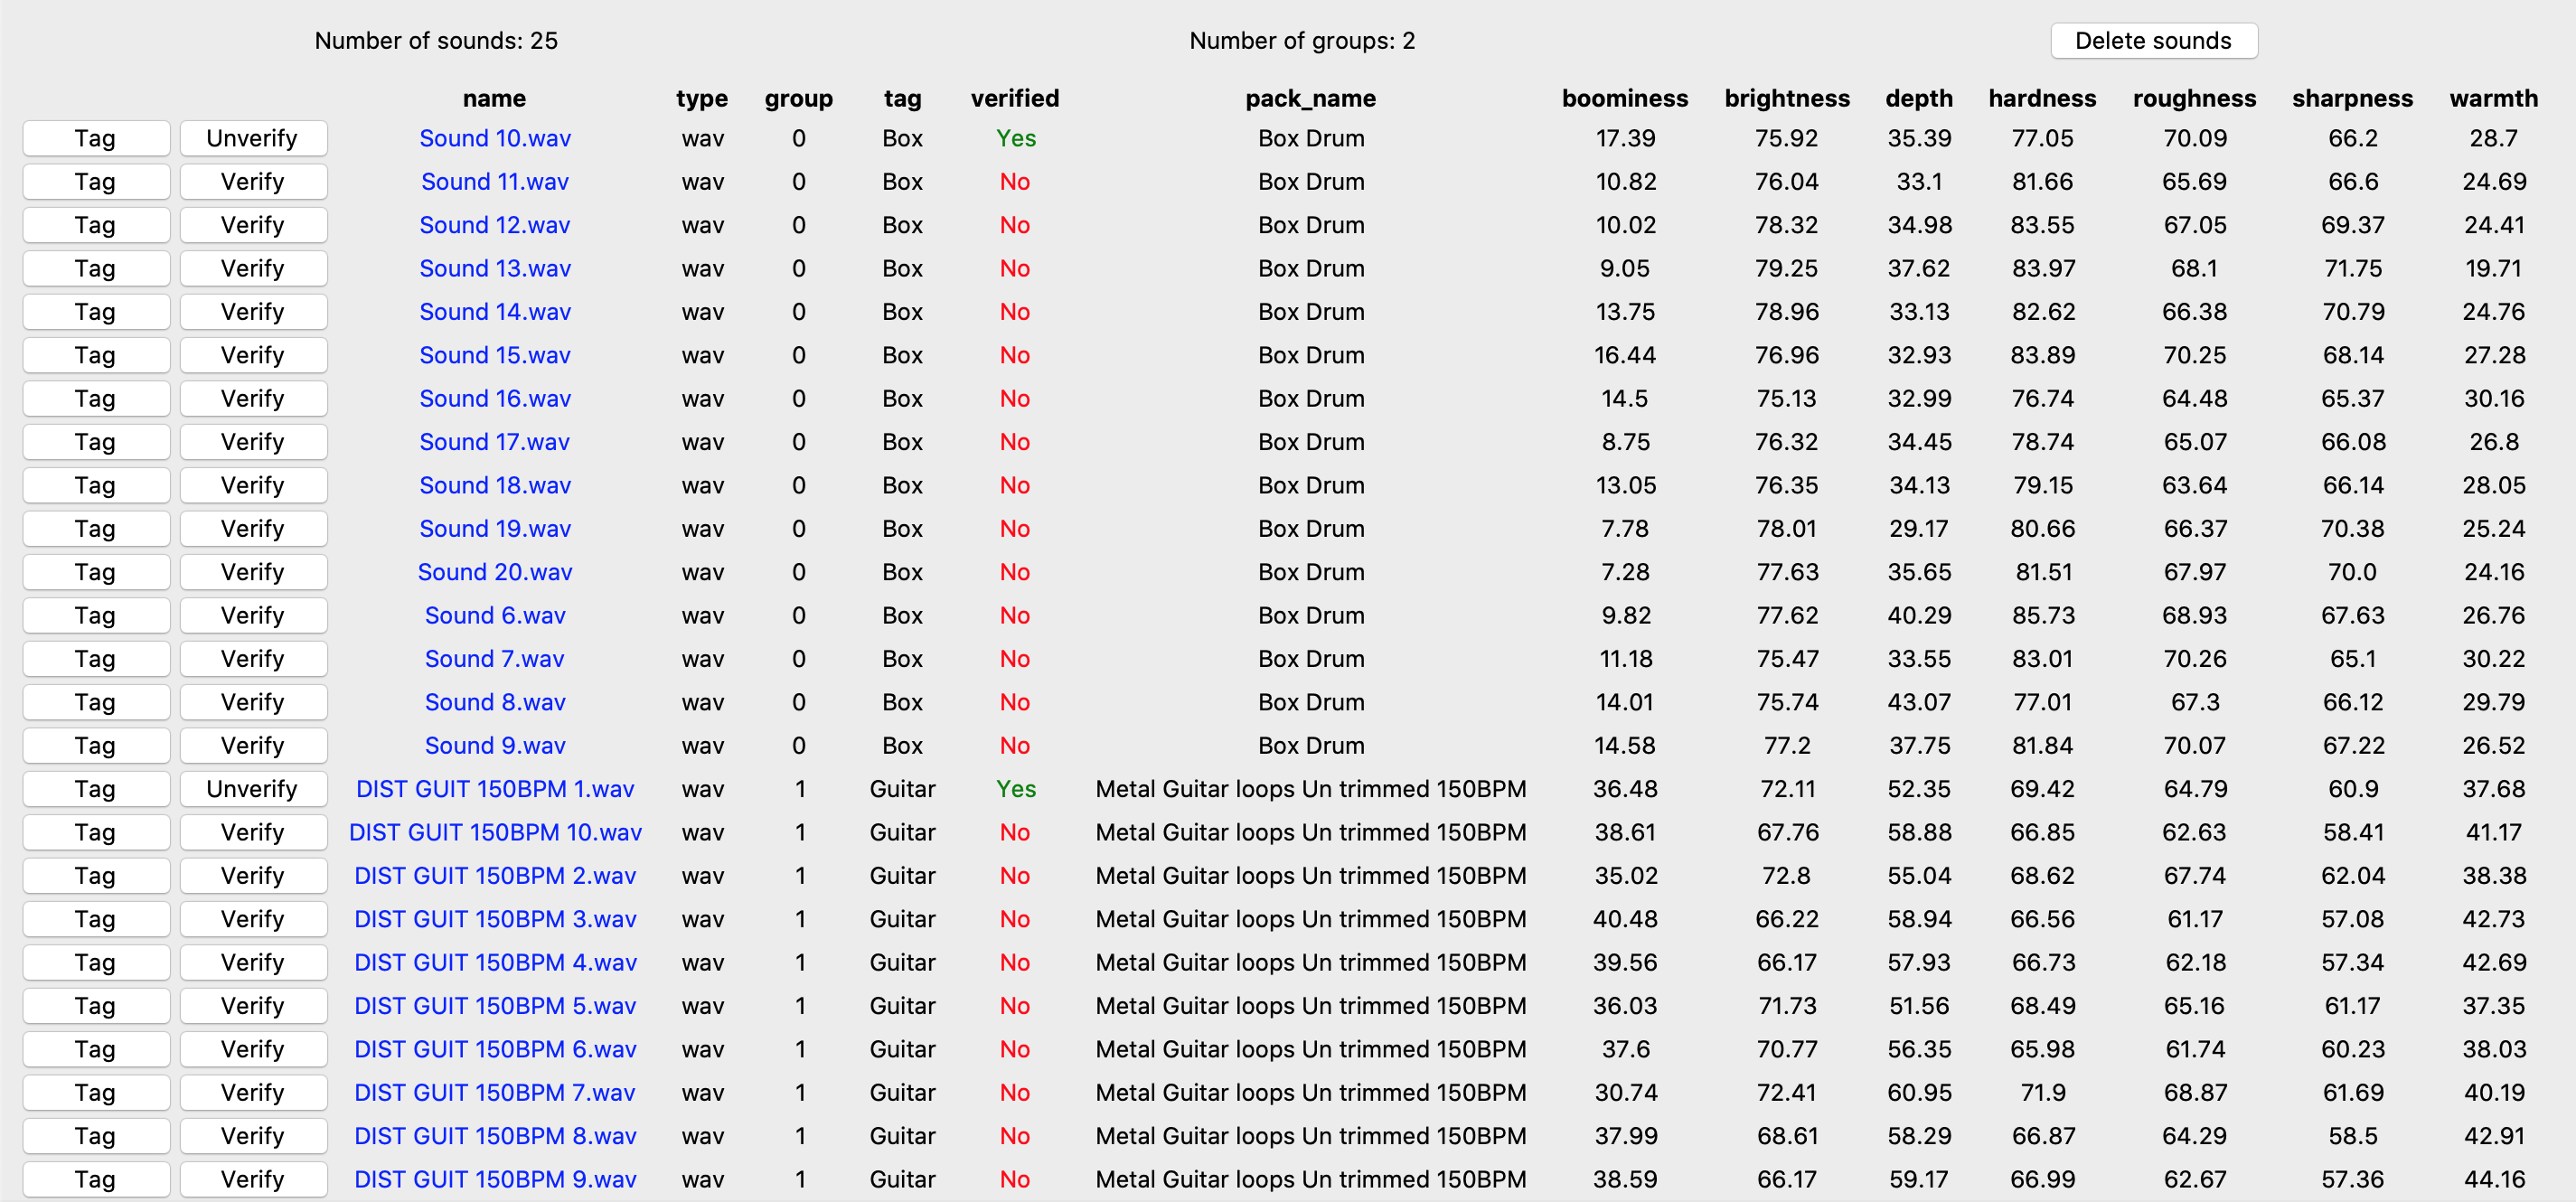
\includegraphics[width=\textwidth]{figures/case_1/finalized}
    \caption{Case 1 test data finalized.}\label{fig:case_1/finalized}
\end{figure}
\clearpage

\newpage\section{Case 2 – Divergence}
The test data in the next use case incorporates sounds from two related packs, both having 15 sound snippets each played on a stringed instrument. The goal will be the same as in the first example: tag the two packs according to the object producing the sounds.

The first pack, \emph{Fretless Bass}, has tracks that are all played on a Harley Benton B-550FL fretless bass without any effects added, but with the selected pickup altering. The \emph{Nylon Guitar Single Notes} pack lacks a description, but the sounds are what the title describes, and make up the second portion of the sounds used in this example. Adding the sounds to the application categorizes most sounds accurately, but some of the guitar sounds end up in the bass group. Labeling the two groups with their relevant tag – \textbf{Bass} for the first pack and \textbf{Guitar} for the latter – illustrates this divergence more clearly.
\begin{figure}[ht]
    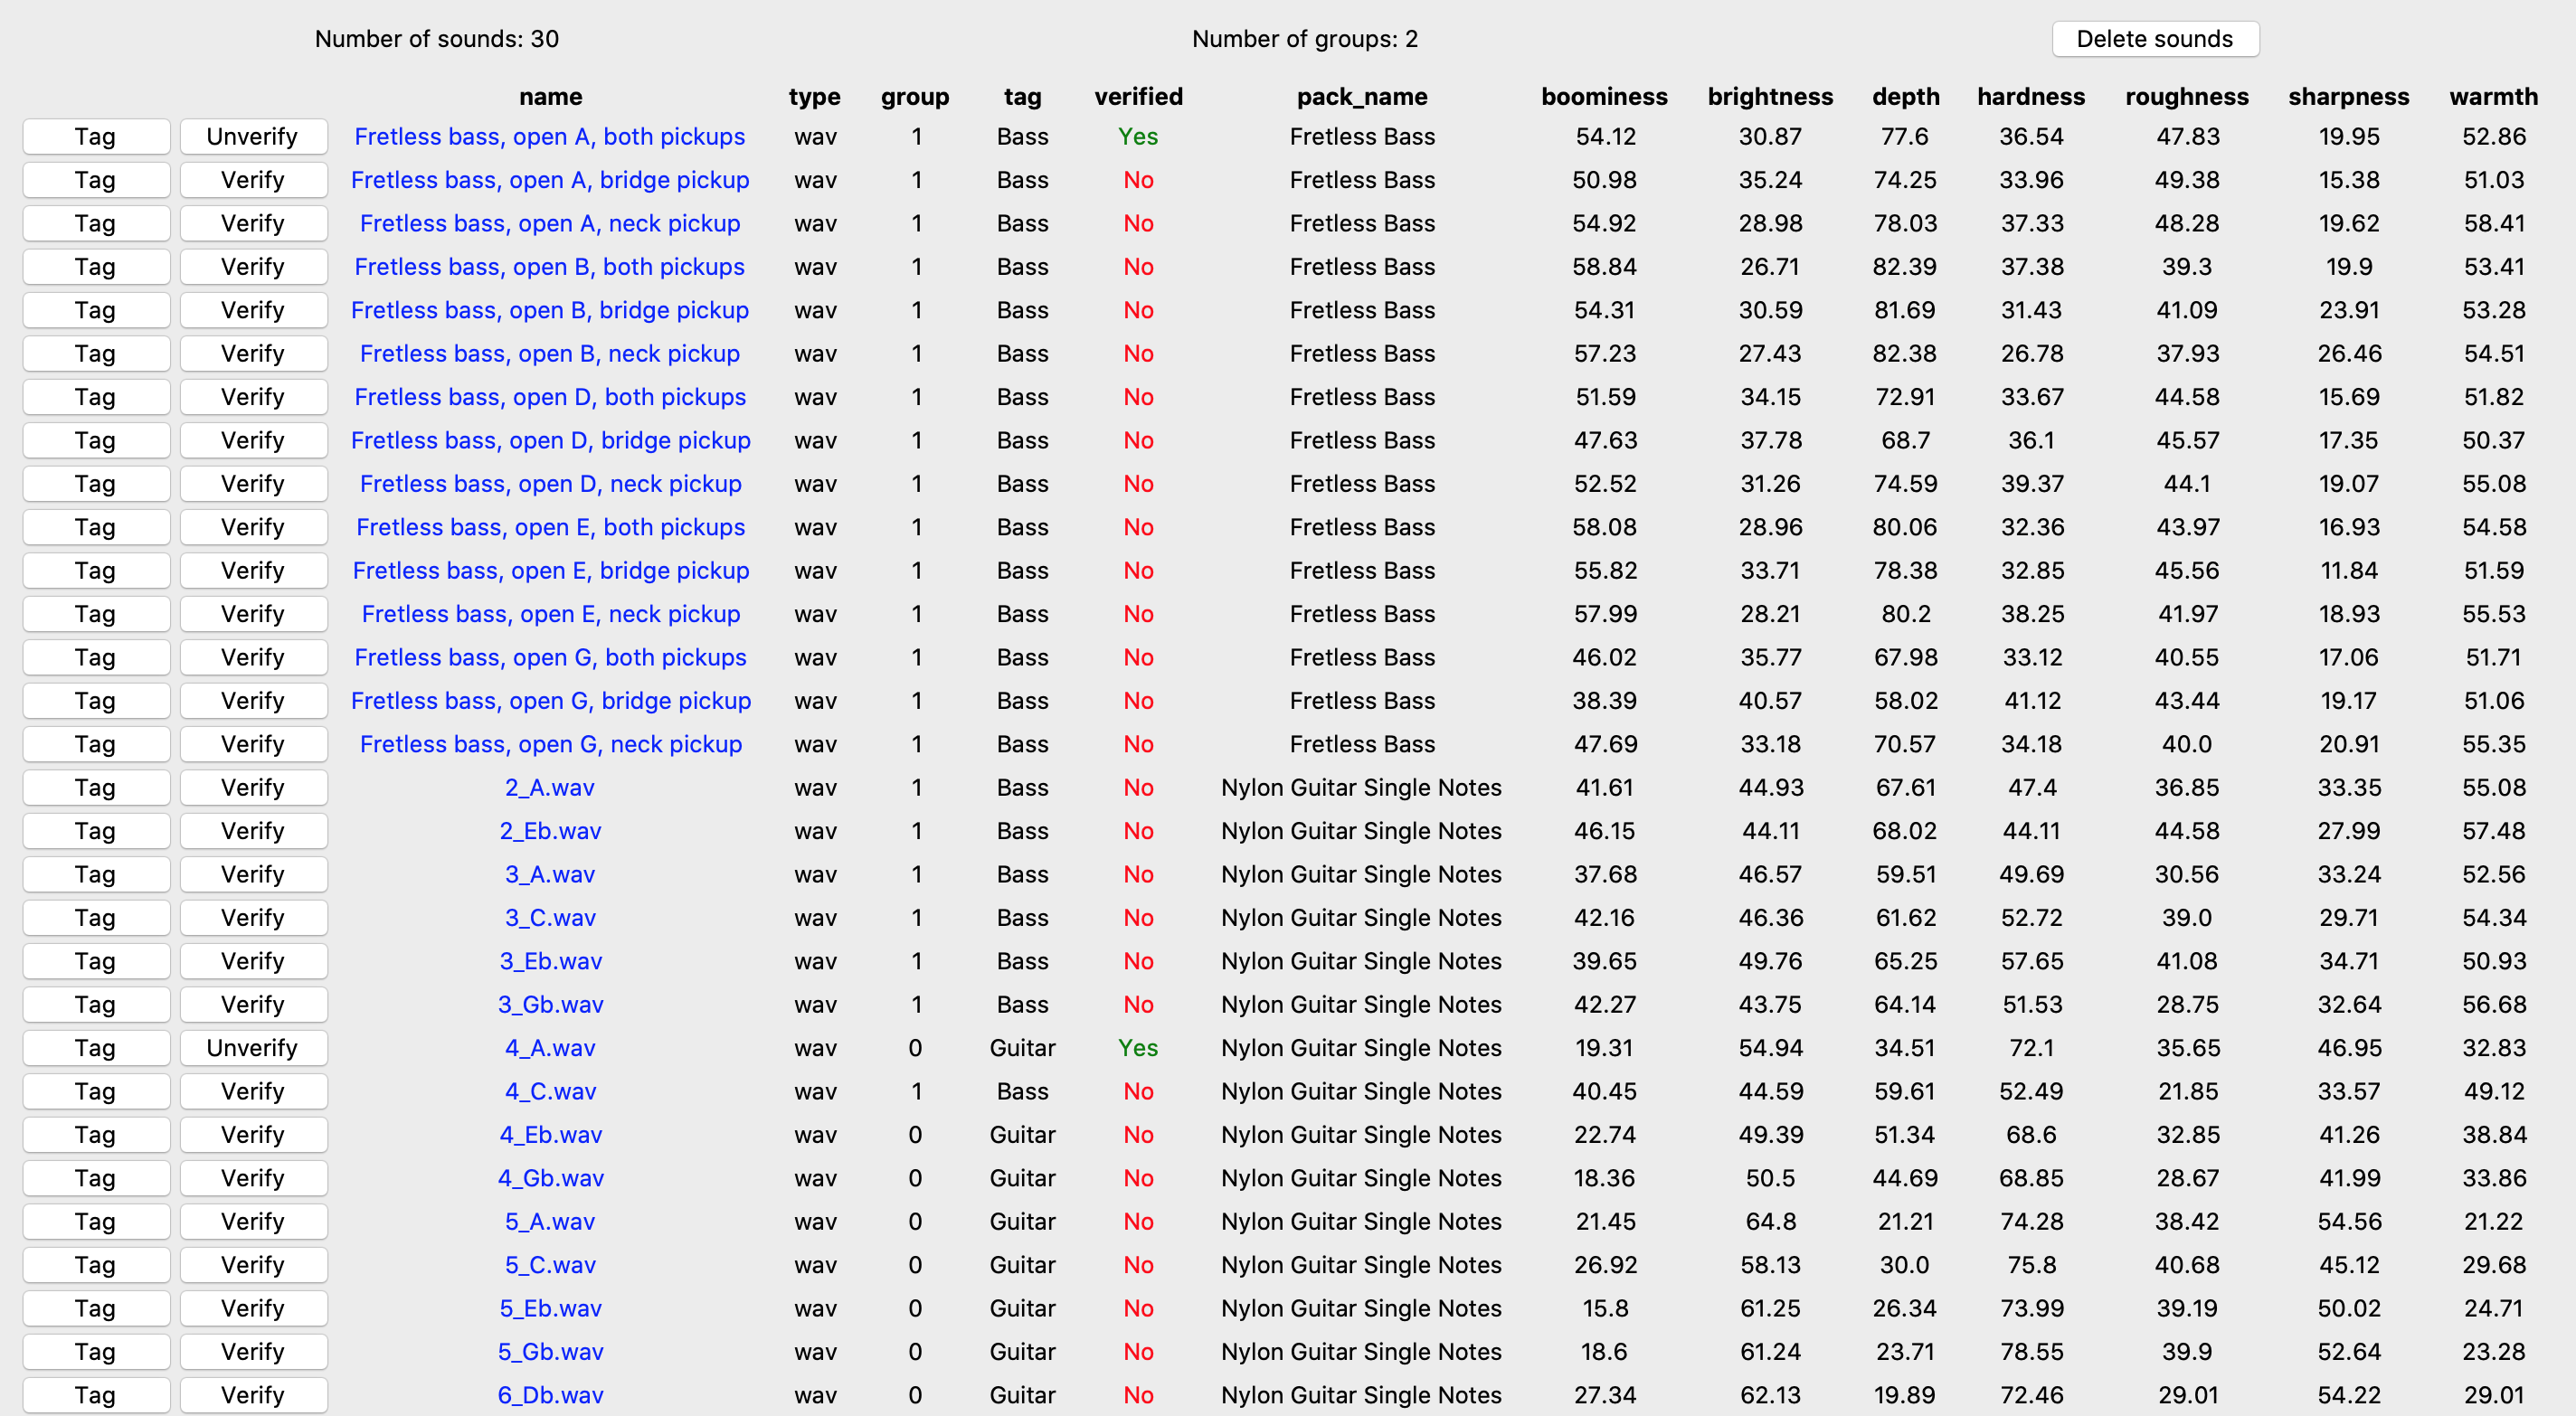
\includegraphics[width=\textwidth]{figures/case_2/initial}
    \caption{Case 2 test data loaded and initially tagged.}\label{fig:case_2/initial}
\end{figure}

This unfinished distribution is a by-product of the groups' correlation to one another and how the sounds themselves are situated. By comparing the ranges for the timbral characteristic values listed in \cref{tab:case_2} with the ones from \cref{tab:case_1} in the first example, it is evident that the test data for the current use case consists of sounds more spread out, at least according to how the program distributes them.
\begin{table}[ht]
    \caption[Case 2 timbral characteristics max and min ranges]{Case 2 timbral characteristics maximum and minimum value ranges}\label{tab:case_2}
    \begin{tabular*}{\textwidth}{@{\extracolsep{\fill}}lrr}
        \toprule
        & \emph{Fretless Bass} & \emph{Nylon Guitar Single Notes} \\
        \midrule
        \textbf{boominess} & 20.45 & 30.35 \\
        \textbf{brightness} & 13.86 & 21.05 \\
        \textbf{depth} & 24.36 & 48.13 \\
        \textbf{hardness} & 14.35 & 34.45 \\
        \textbf{roughness} & 11.46 & 22.73 \\
        \textbf{sharpness} & 14.62 & 26.57 \\
        \textbf{warmth} & 8.04 & 36.26 \\
        \midrule
        Average & 15.31 & 31.36 \\
        \bottomrule
    \end{tabular*}
\end{table}

\newpage Finishing this example can be done in several ways, but resolving an average score involves trying every path available. Because the sound pool is quite small in this example, it is possible to check each path individually. Coincidentally, all alternatives take \textbf{two corrections} to achieve the goal of one tag per sound pack.
\begin{figure}[ht]
    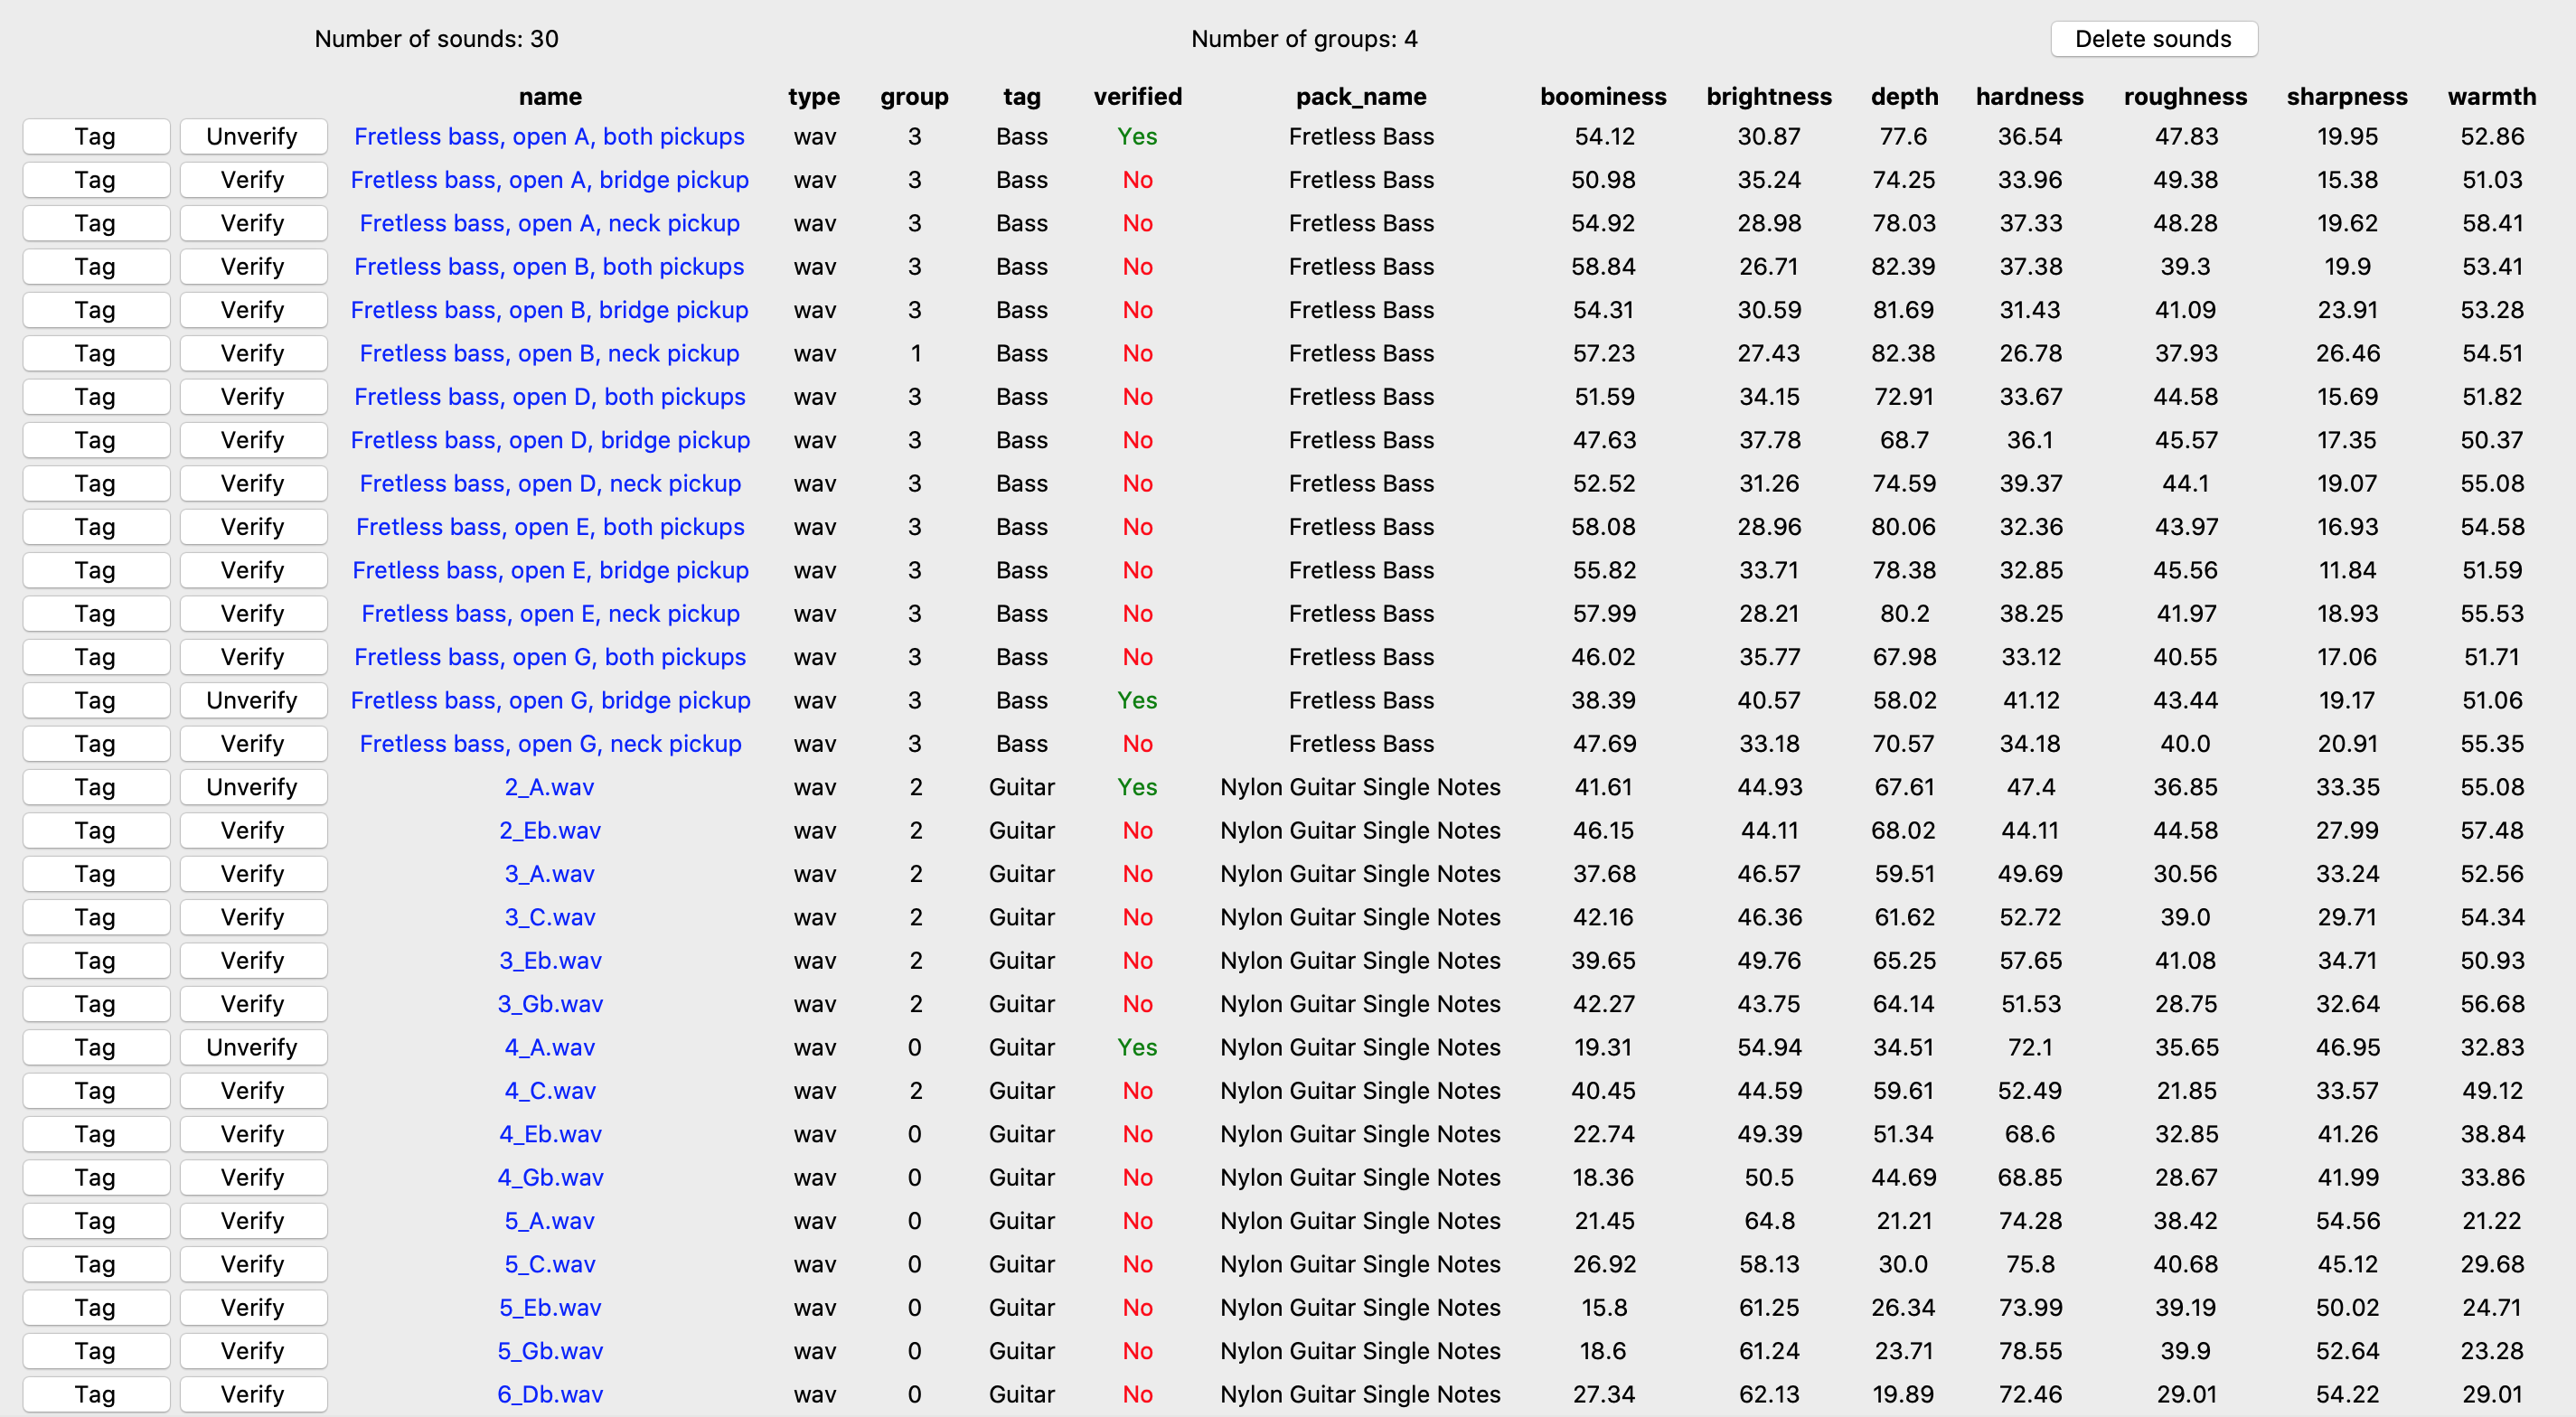
\includegraphics[width=\textwidth]{figures/case_2/finalized}
    \caption{Case 2 finalized in one of several different ways.}\label{fig:case_2/finalized}
\end{figure}
\clearpage

\newpage\section{Case 3 – Scope}\label{sec:case_3}
An intriguing quality of the \gls{ml} algorithms used to tag sounds automatically in the application is how they execute differently depending on the scope of the data points in a given input series. Stripping the sound pool in the first example – where the application immediately groups the loaded samples correctly – to a single pack, one could expect the program to identify that pack as a single group.

That is not quite the case, as can be seen in \cref{fig:case_3/demo-1}, where the \emph{Metal Guitar loops Un trimmed 150BPM} pack is inserted by itself. This perchance unexpected event happens due to the nature of how the clustering algorithms function when handling differently sized and spread out data sets. One way to potentially regulate this action would be to fine-tune the precision at which the application generates the sound groupings. The tolerance value is such a calibration but, although publicly available for reconfiguration as a function argument labeled \emph{tol}~\cite{mean_shift:api, k-means:api}, remains untouched and set to its default behavior in this implementation. Tweaking this attribute could help the program adjust to certain situations better and possibly improve the performance for specific cases; the further work segment (\cref{sec:further_work}) examines this proposal further.
\begin{figure}[ht]
    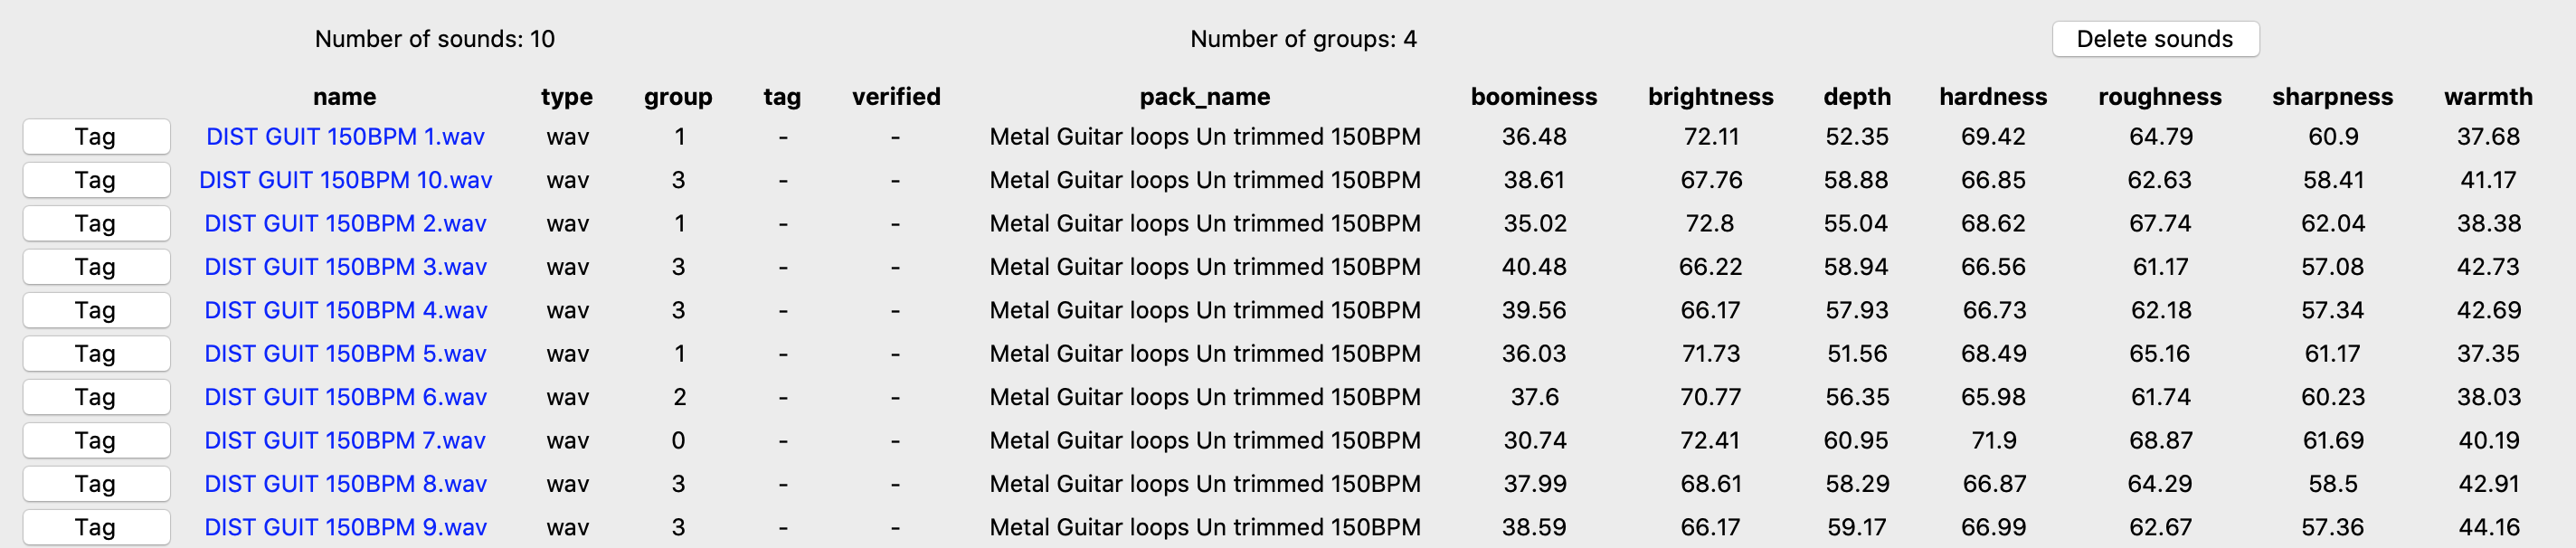
\includegraphics[width=\textwidth]{figures/case_3/demo-1}
    \caption{Pack from Case 1 loaded separately into the application.}\label{fig:case_3/demo-1}
\end{figure}

Expanding on this topic: when duplicating a single sound and adding both the original and copied one to the application, the two sounds will end up belonging to the same group. Furthermore, as accomplished in \cref{fig:case_3/demo-2} by copying and modifying an individual Freesound metadata file, if two sounds differ even in a single magnitude for one of the timbral attributes, the resulting sum of groups will be two.
\begin{figure}[ht]
    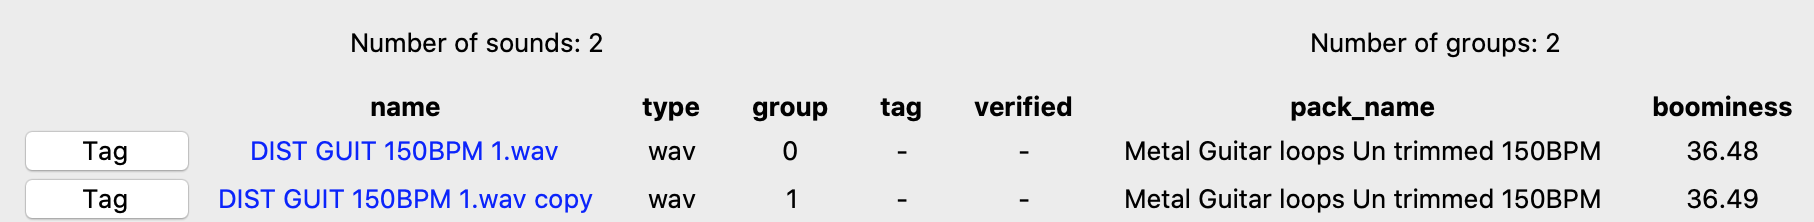
\includegraphics[width=\textwidth]{figures/case_3/demo-2}
    \caption{A single sound plus its modified clone loaded into the application.}\label{fig:case_3/demo-2}
\end{figure}

\newpage One can think of this concept as a `zoom effect' in the dimensional space where the resulting picture is the same whether the parameters are large or small as long as the proportions remain constant. Reducing the dimensions of predicted timbral characteristics from seven to two enables a relatively effective visualization of this type of proportion-based groupings relative to the volume of the sounds added to the program. In two dimensions, this means that the size of the \(x\) and \(y\) values (for example, \emph{boominess} and \emph{brightness}) is redundant when distributing the groups, and only the relative distance between the data points on the coordinate axes is of importance. This phenomenon is also, in some instances, comparable to the \emph{Droste effect}, where a picture appears within itself one or multiple times, as shown in \cref{fig:case_3/demo-3}.
\begin{figure}[ht]
    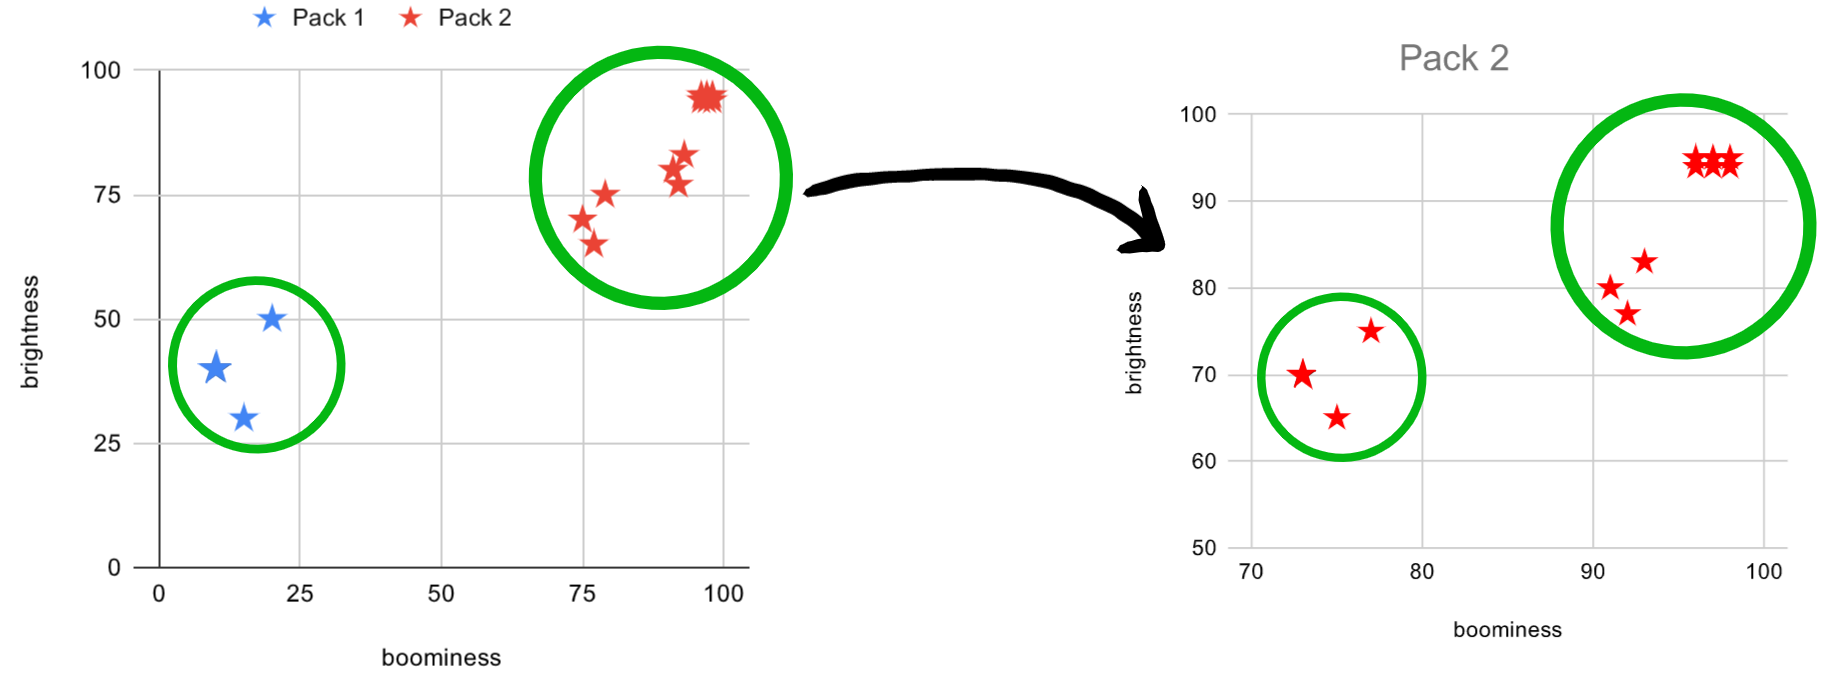
\includegraphics[width=\textwidth]{figures/case_3/demo-3}
    \caption[An illustration of the \emph{Droste effect} in the application.]{An illustration of the \emph{Droste effect} in the application when changing the scope for sounds added to the program. The green circles represent the determined groups found by the application. Pack 2 has the same layout of sounds in itself as it has with Pack 1, hence the groupings being the same when processed together or Pack 2 by itself, even though the scale changes in the two pictures.}\label{fig:case_3/demo-3}
\end{figure}
\clearpage

\newpage\section{Case 4 – Scalability}
The last example mimics a more realistic usage of the application, with six different packs on a smaller scale, forming a total of 30 sounds. The test data is made up of instrumental, electronic, and ambient sounds, stretching over a broader sound domain than previous examples. As before, the goal is to give every sound in each pack a descriptive group tag that corresponds to its sounds' source.

The first pack, \emph{A Harpsicord Dream}~\cite{pack:1793}, consists of harp-like glissandos played on a Roland XP-10 keyboard. The two next packs used, \emph{Basic Tech-Trance}~\cite{pack:1292} and \emph{Bass Bars 1}~\cite{pack:1254}, have beats that would suit as a foundation for loops in techno songs. \emph{Sharpening Knives}~\cite{pack:2280} and \emph{Static and Radio Sounds}~\cite{pack:1867} contain samples of audio from everyday life. \emph{Tom-Tom Grooves}~\cite{pack:2918} is the last pack included in the test data and has short loop-friendly drum rhythms. It is noticeable when examining the averages in \cref{tab:case_4} that the estimated timbral characteristics map some of the chosen packs as more compact and other as more spread out.

When handing the test data to the application for analysis, it does a decent job of organizing the sounds; \cref{fig:case_4/initial} displays this initial state. The number of groups predicted is slightly modest, consequently mixing and joining some packs together. Reaching a finalized state of \cref{fig:case_4/finalized} takes an unfixed amount of user interactions – explained in \cref{sec:measurement}. Because the number of revisions has grown compared to other use cases, it is laborious to cover every alternative and, therefore, difficult to work out an exact median value for the number of alterations needed.

\begin{table}[ht]
    \caption[Case 4 timbral characteristics max and min ranges]{Case 4 timbral characteristics maximum and minimum value ranges}\label{tab:case_4}
    \begin{tabular*}{\textwidth}{@{\extracolsep{\fill}}lrr}
        \toprule
        \multicolumn{3}{c}{\textbf{\underline{Instrumental}}} \\
        & \emph{A Harpsicord Dream} & \emph{Tom-Tom Grooves} \\
        \midrule
        \textbf{boominess} & 9.69 & 3.34 \\
        \textbf{brightness} & 8.40 & 0.87 \\
        \textbf{depth} & 11.64 & 2.06 \\
        \textbf{hardness} & 18.10 & 3.19 \\
        \textbf{roughness} & 2.27 & 2.27 \\
        \textbf{sharpness} & 7.57 & 2.44 \\
        \textbf{warmth} & 9.87 & 1.51 \\
        \midrule
        Average & 9.65 & 2.24 \\
        \midrule \\
        \multicolumn{3}{c}{\textbf{\underline{Electronic}}} \\
        & \emph{Basic Tech-Trance} & \emph{Bass Bars 1} \\
        \midrule
        \textbf{boominess} & 11.63 & 9.13 \\
        \textbf{brightness} & 32.19 & 10.78 \\
        \textbf{depth} & 9.18 & 9.21 \\
        \textbf{hardness} & 25.27 & 10.53 \\
        \textbf{roughness} & 27.99 & 5.64 \\
        \textbf{sharpness} & 29.00 & 7.38 \\
        \textbf{warmth} & 26.97 & 3.68 \\
        \midrule
        Average & 23.18 & 8.05 \\
        \midrule \\
        \multicolumn{3}{c}{\textbf{\underline{Ambient}}} \\
        & \emph{Sharpening Knives} & \emph{Static and Radio Sounds} \\
        \midrule
        \textbf{boominess} & 24.52 & 5.77 \\
        \textbf{brightness} & 5.45 & 3.95 \\
        \textbf{depth} & 18.77 & 17.58 \\
        \textbf{hardness} & 13.96 & 15.38 \\
        \textbf{roughness} & 10.40 & 6.76 \\
        \textbf{sharpness} & 13.14 & 9.97 \\
        \textbf{warmth} & 3.17 & 12.56 \\
        \midrule
        Average & 12.77 & 10.28 \\
        \bottomrule
    \end{tabular*}
\end{table}
\clearpage

\begin{figure}[ht]
    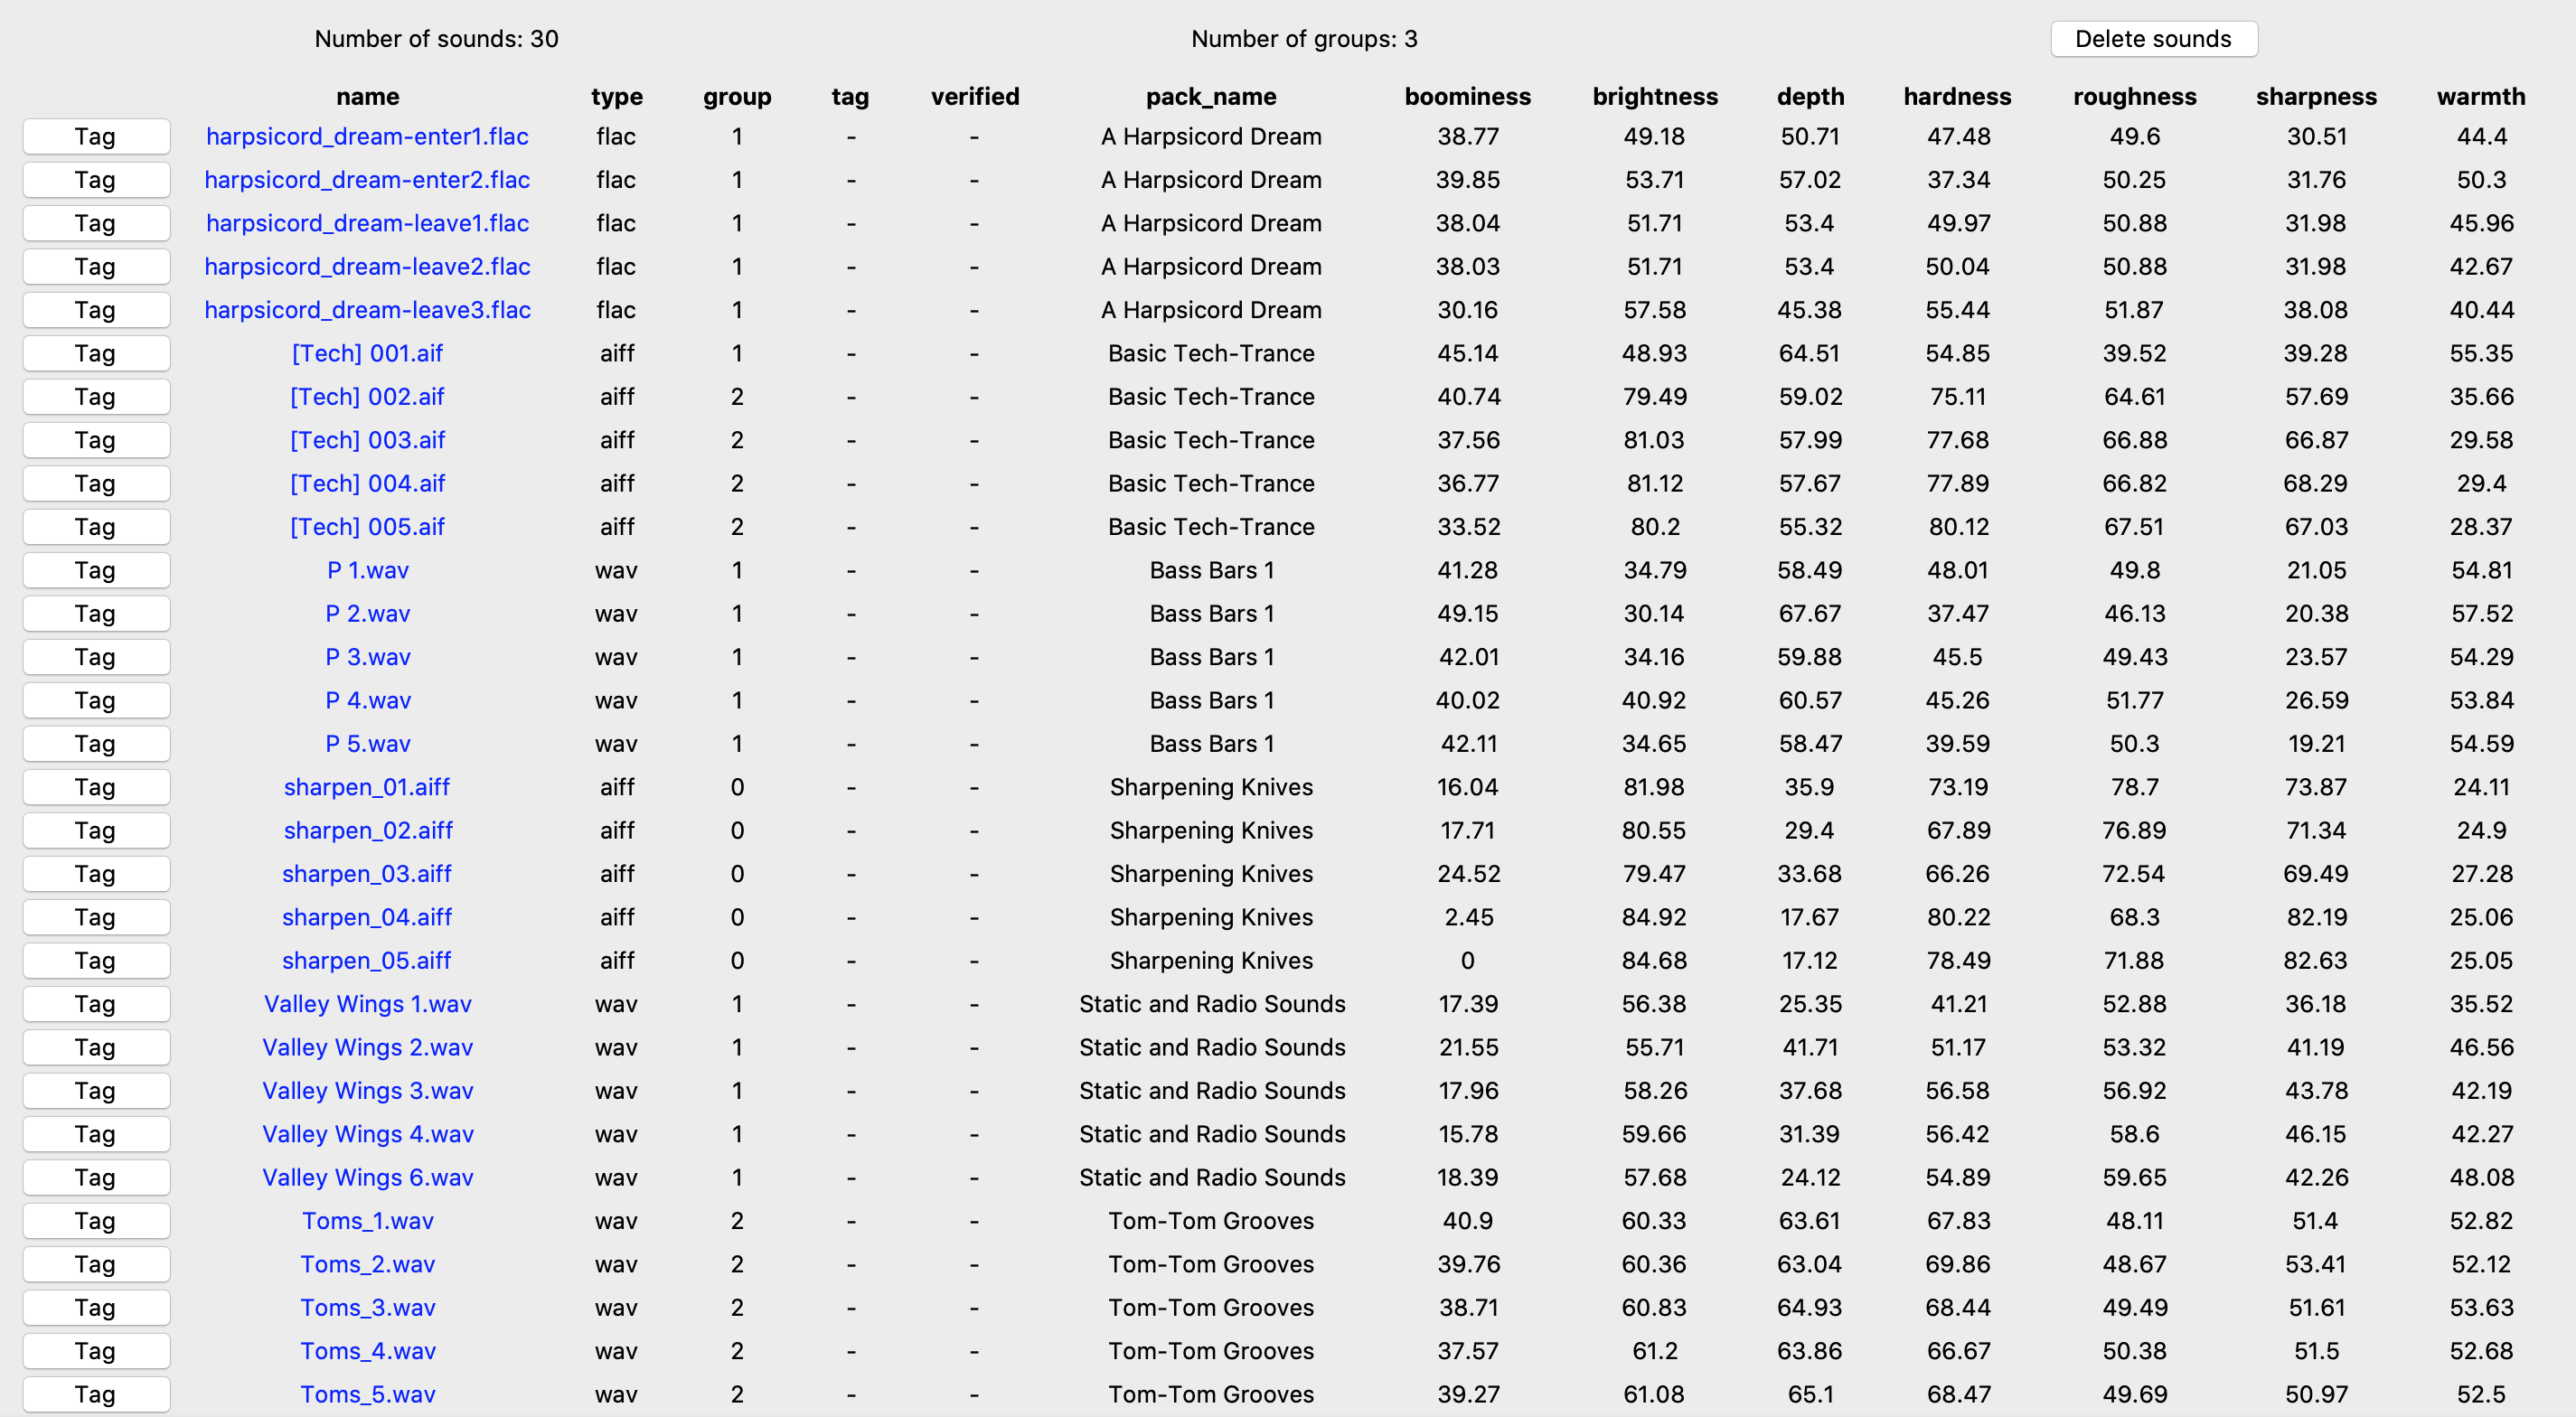
\includegraphics[width=\textwidth]{figures/case_4/initial}
    \caption{Case 4 test data initially loaded into the application.}\label{fig:case_4/initial}
\end{figure}

\begin{figure}[ht]
    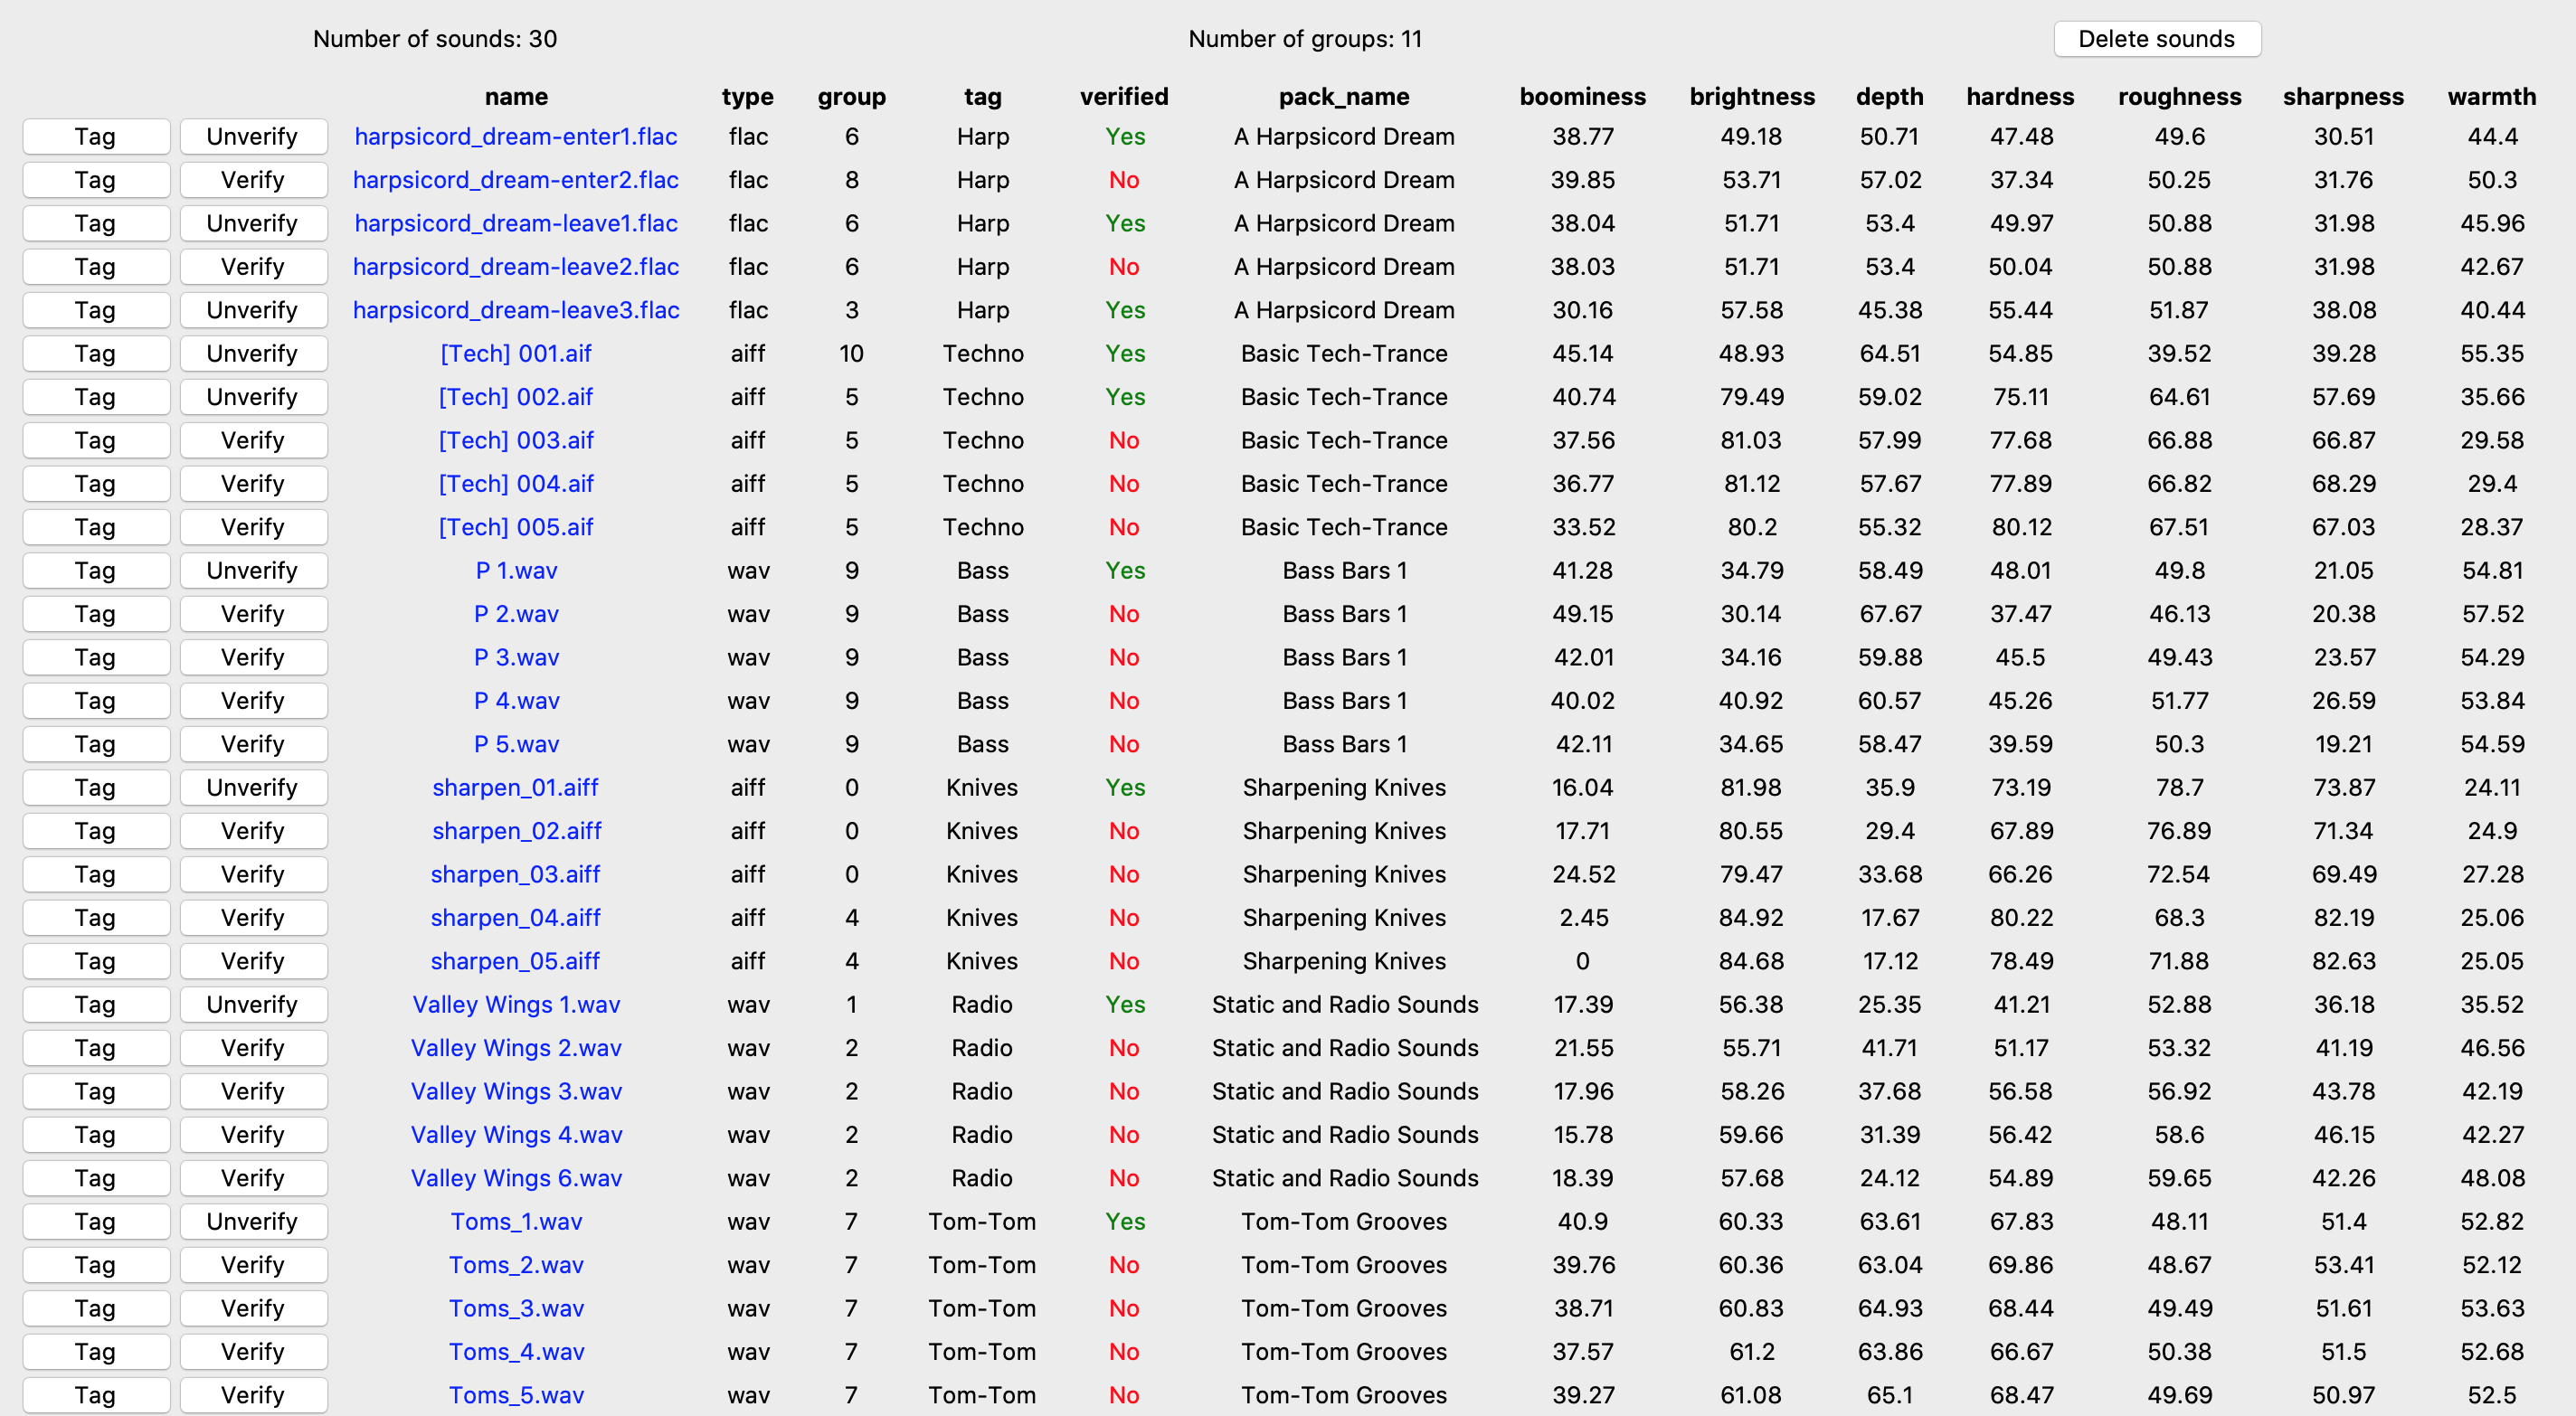
\includegraphics[width=\textwidth]{figures/case_4/finalized}
    \caption{Case 4 finalized in one of several different ways.}\label{fig:case_4/finalized}
\end{figure}

\egroup{}